\begin{frame}
  \frametitle{Modello 1D}
  \begin{columns}

    \column{.5\textwidth}
    Equazione di Langevin:
      \[ x_i^{n+1} = x_i^n + v\mathrm{d}t + \sqrt{2D\cdot\mathrm{d}t}\zeta \]
      Nascita e morte: processi stocastici

    \column{.5\textwidth}
    Validazione delle condizioni al contorno \\
    (solo advezione + diffusione):
    \begin{figure}[!htb]
      \centering
      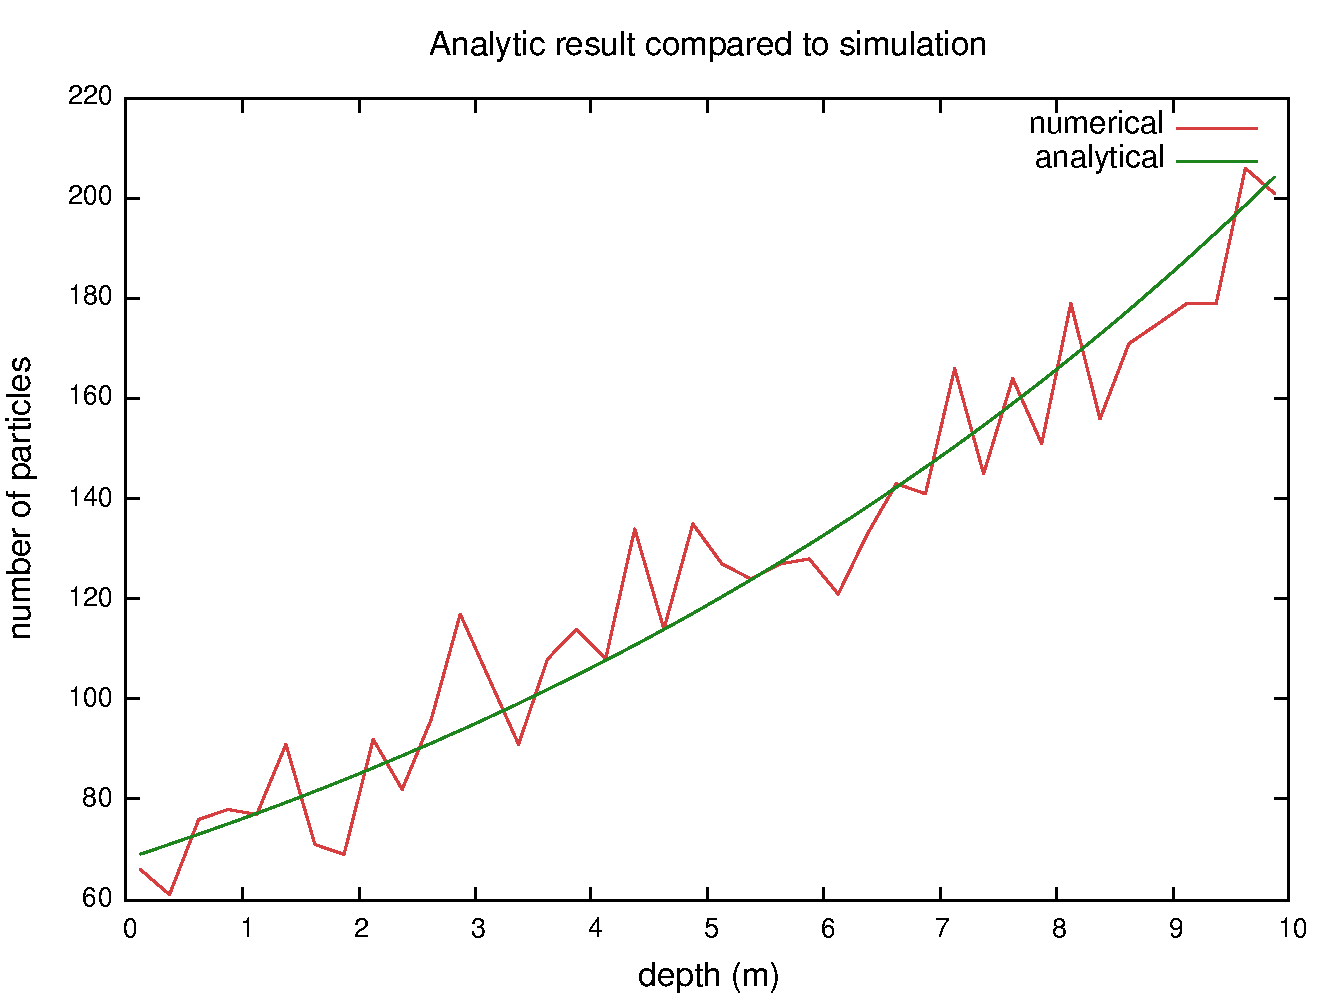
\includegraphics[width=\textwidth]{../prg/numerical_1D/stoc_fin_diff_oop/growth_test/cfr_stoc_refl.pdf}
    \end{figure}

  \end{columns}
\end{frame}

\begin{frame}
  \frametitle{Modello 1D}
  \begin{columns}

    \column{.3\textwidth}
    Riproduzione dei risultati di Huisman
    \begin{figure}[!htb]
      \centering
      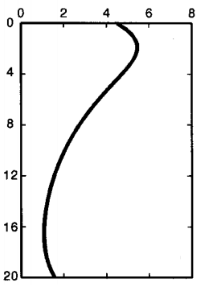
\includegraphics[width=\textwidth]{../img/huisman_profile}
    \end{figure}

    \column{.7\textwidth}
    \begin{figure}[!htb]
      \centering
      \includegraphics[width=.6\textwidth]{../prg/numerical_1D/stoc_fin_diff_oop/results/profile_example}
    \end{figure}

  \end{columns}
\end{frame}

\begin{frame}
  \frametitle{Modello 1D}
  \begin{columns}

    \column{.3\textwidth}
    Riproduzione dei risultati di Huisman (no-flux)
    \begin{figure}[!htb]
      \centering
      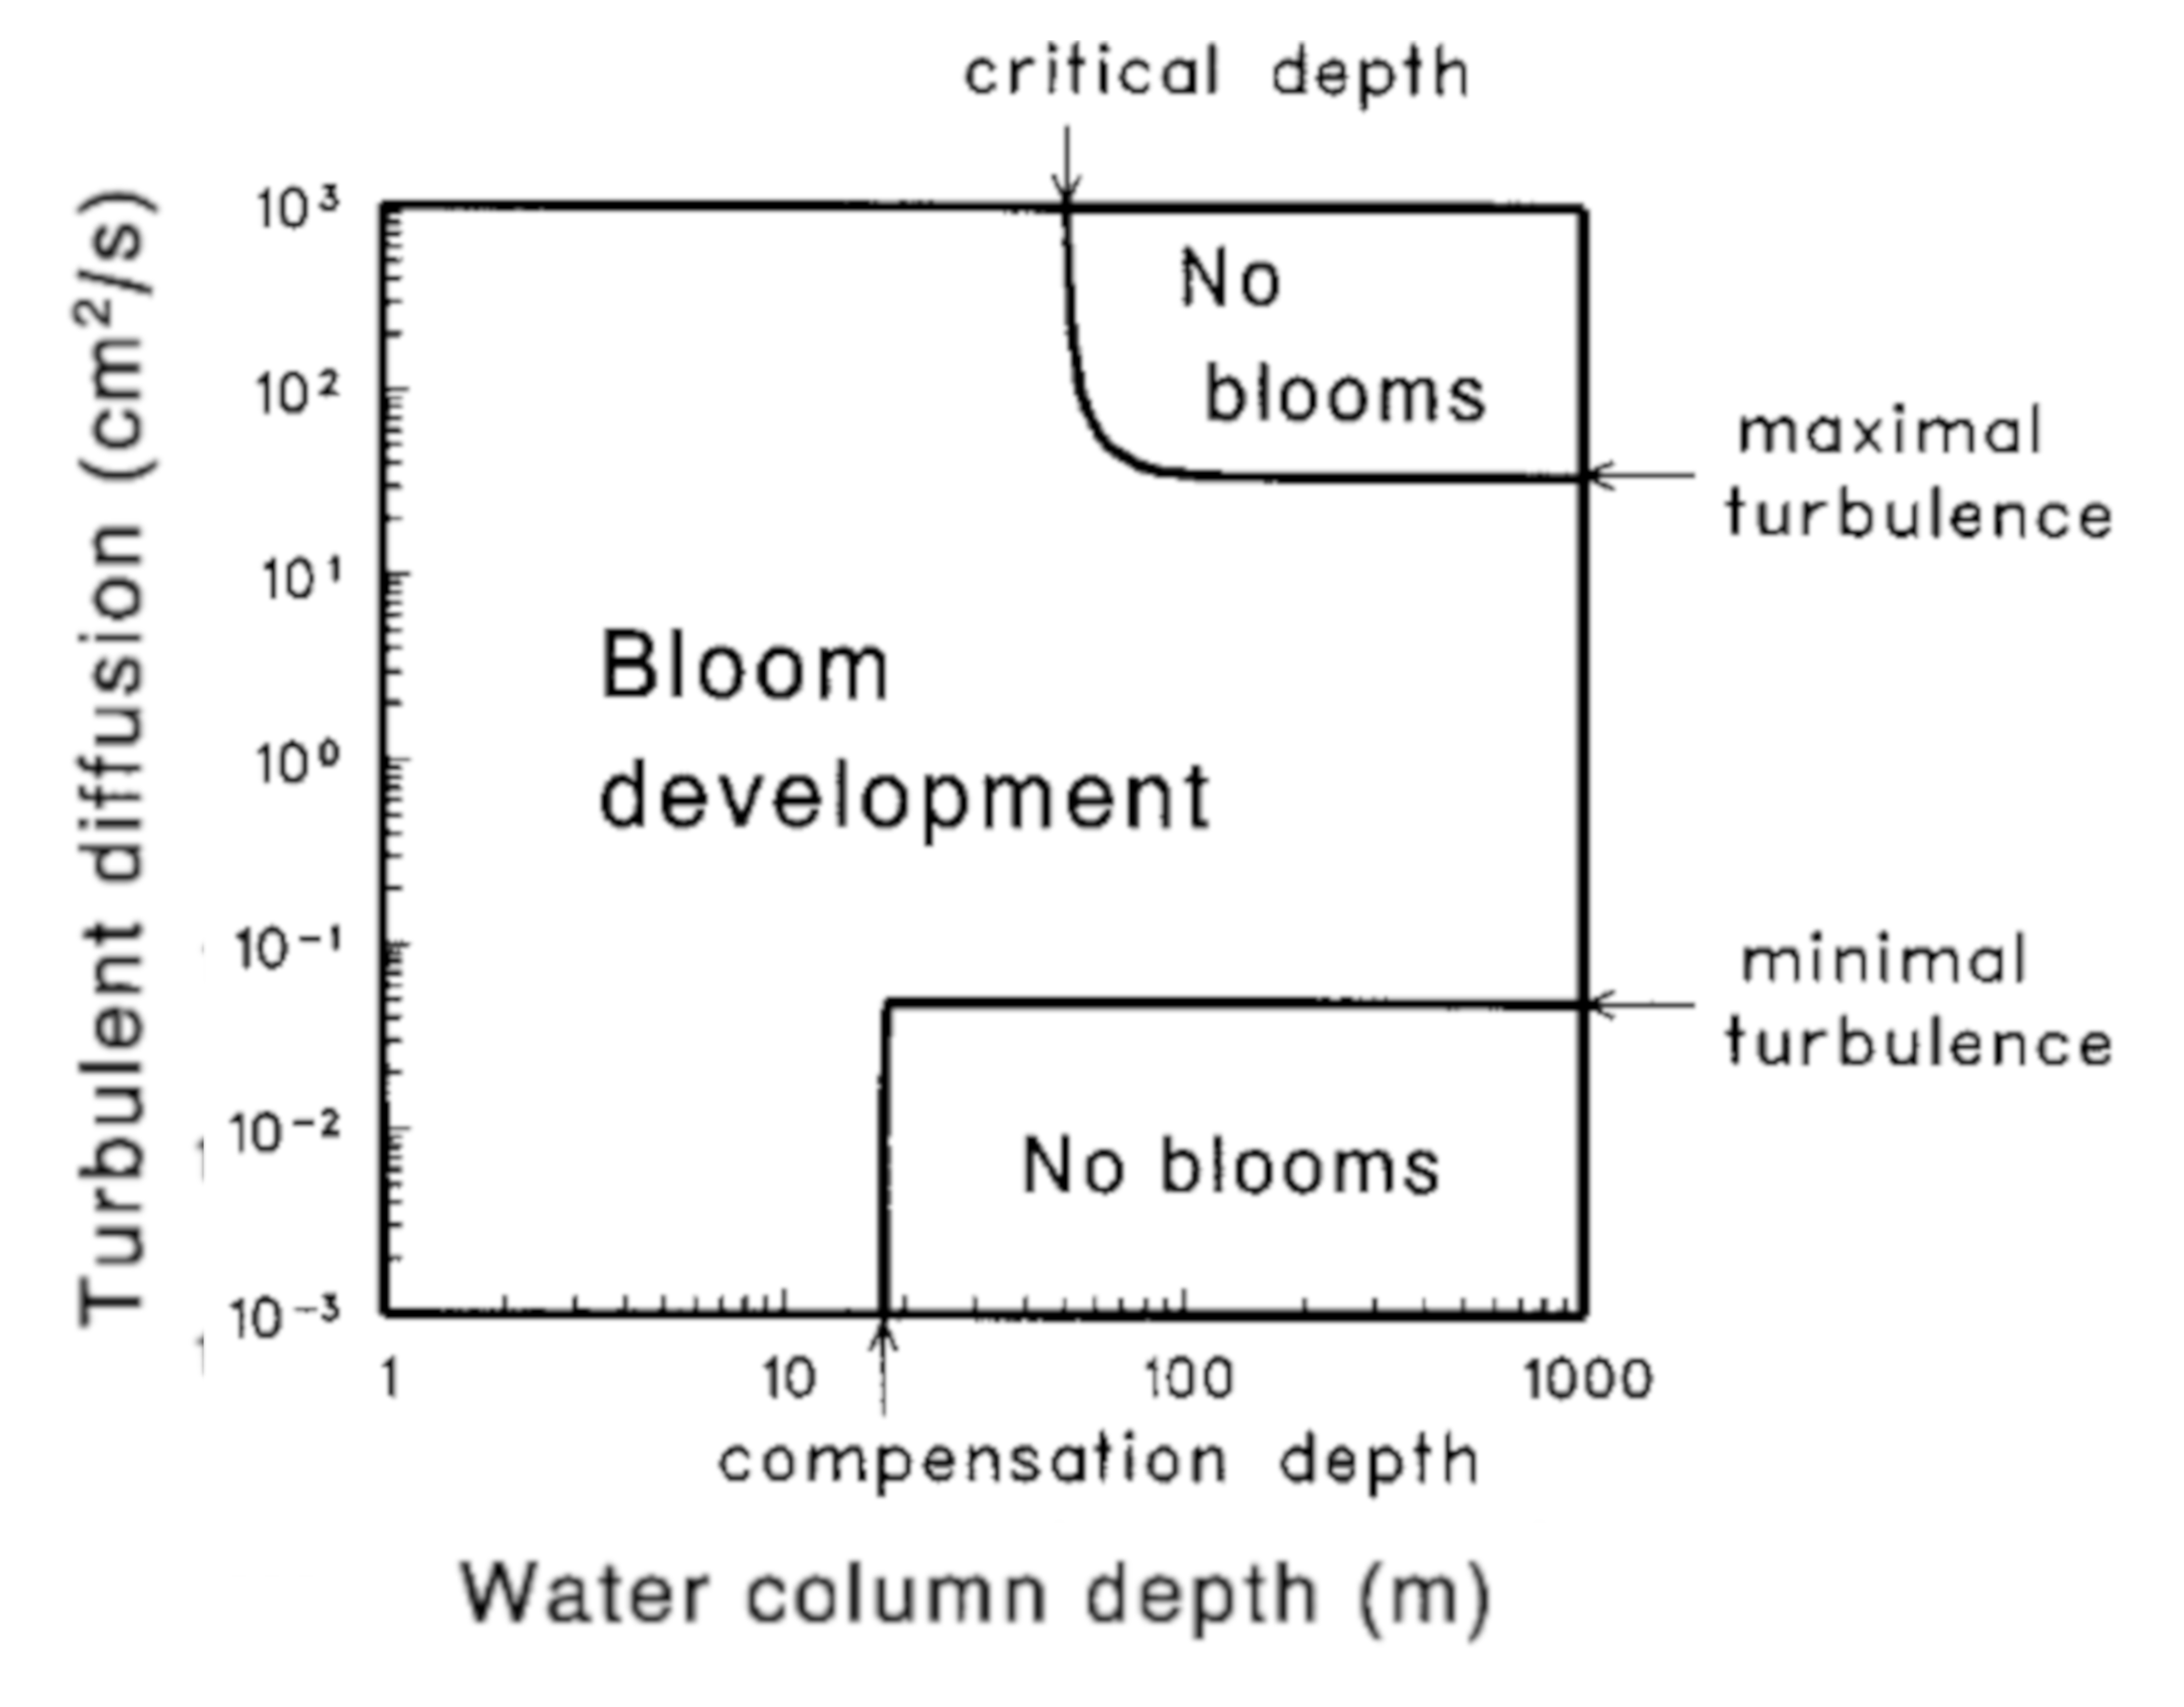
\includegraphics[width=\textwidth]{../img/huisman_lowvel_minimal}
    \end{figure}

    \column{.7\textwidth}
    \begin{figure}[!htb]
      \centering
      \includegraphics[width=\textwidth]{../prg/numerical_1D/stoc_fin_diff_oop/results/refl_bound/bloom}
    \end{figure}

  \end{columns}
\end{frame}

\begin{frame}
  \frametitle{Modello 1D}
  \begin{columns}
    
    \column{.3\textwidth}
    Tempo di vita medio
    \begin{figure}[!htb]
      \centering
      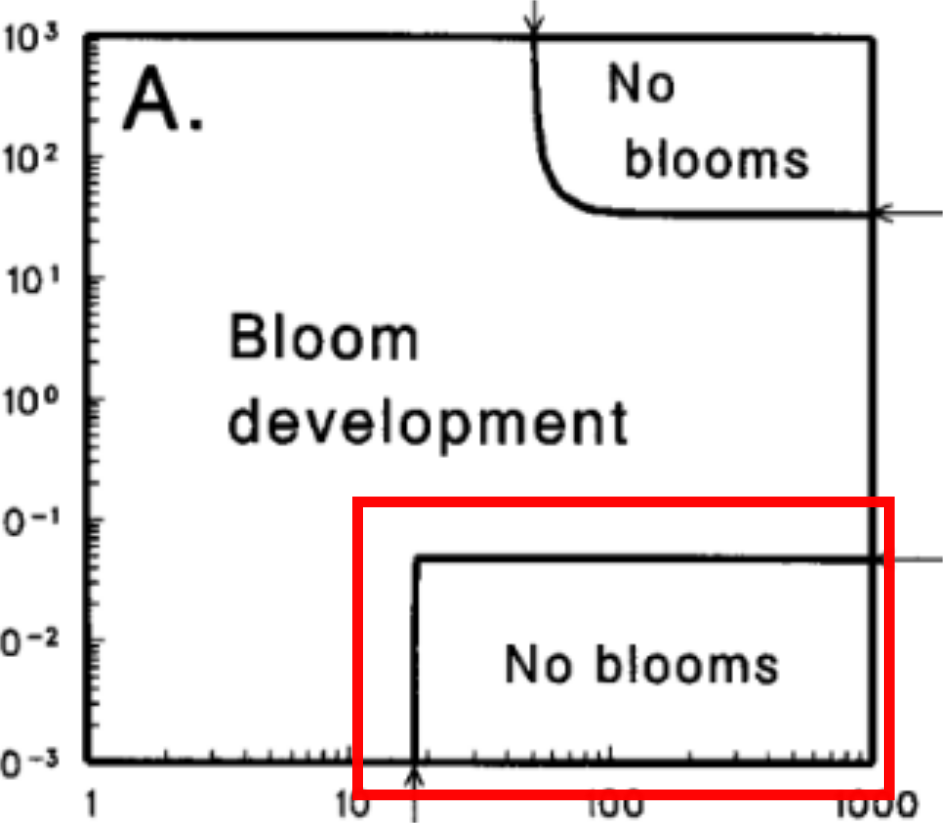
\includegraphics[width=\textwidth]{../img/huisman_lowvel_minimal_zoom}
    \end{figure}
 
    \column{.7\textwidth}
    \begin{figure}[!htb]
      \centering
      \includegraphics[width=\textwidth]{../prg/numerical_1D/stoc_fin_diff_oop/bottom_right_test/bloom_time}
    \end{figure}

  \end{columns}
\end{frame}

%\begin{frame}
%  \frametitle{Modello 1D}
%  \begin{columns}
%
%    \column{.3\textwidth}
%    Riproduzione dei risultati di Huisman: alta velocità di affondamento 
%    \\
%    (no-flux)
%    \begin{figure}[!htb]
%      \centering
%      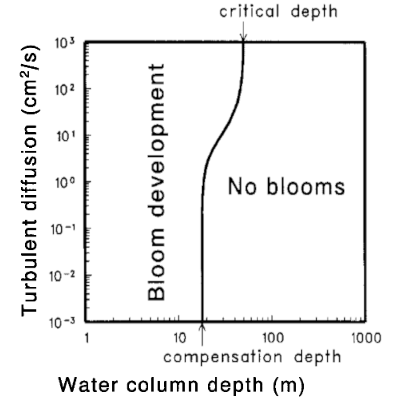
\includegraphics[width=\textwidth]{../img/huisman_hivel_minimal}
%    \end{figure}
%
%    \column{.7\textwidth}
%    \begin{figure}[!htb]
%      \centering
%      \includegraphics[width=\textwidth]{../prg/numerical_1D/stoc_fin_diff_oop/results/high_velocity/bloom}
%    \end{figure}
%
%  \end{columns}
%\end{frame}


\begin{frame}
  \frametitle{Modello 1D}
  \begin{columns}

    \column{.3\textwidth}
    Esplorazione delle condizioni assorbenti
    \begin{figure}[!htb]
      \centering
      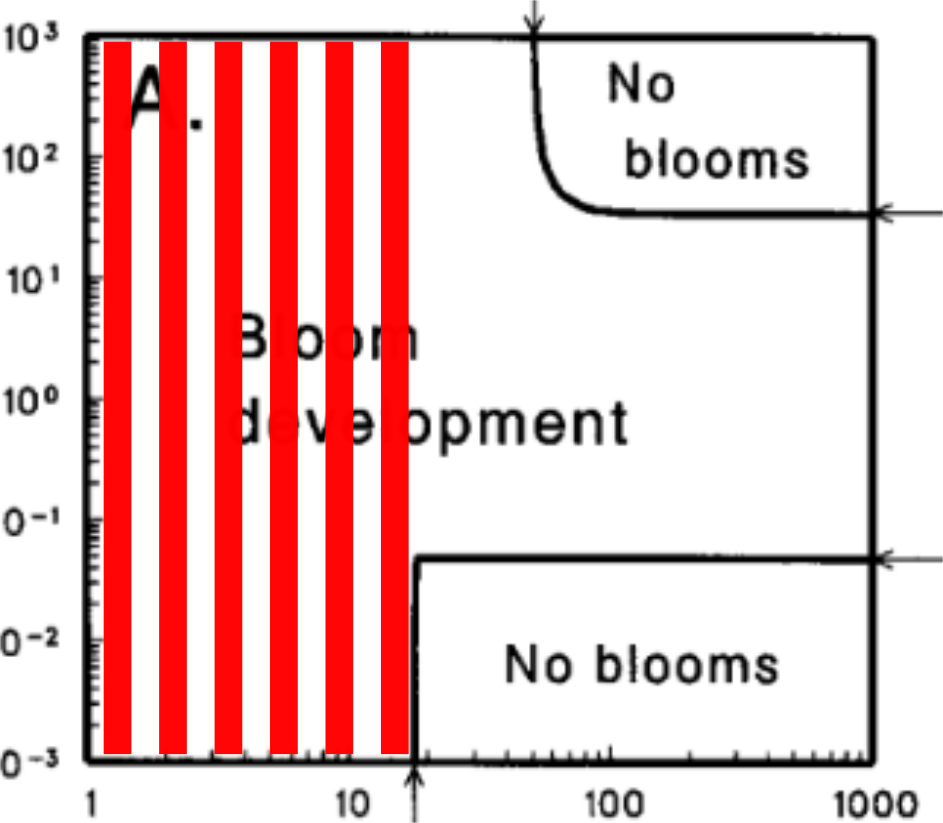
\includegraphics[width=\textwidth]{../img/huisman_lowvel_minimal_absorbing}
    \end{figure}

    \column{.7\textwidth}
    \begin{figure}[!htb]
      \centering
      \includegraphics[width=\textwidth]{../prg/numerical_1D/stoc_fin_diff_oop/results/absorb_bound/bloom}
    \end{figure}

  \end{columns}
\end{frame}


